\newpage
\subsection{Projection des rayons}
\label{subsec:projection}
%%\nameref{Projection des rayons}
Pour projeter les rayons partant du point $Origine\in \mathbb{R}^3$ et de direction $Direction\in \mathbb{R}^3$, on utilise la suite suivante:
$$
(Pos_n)_{n\in \mathbb{N}}=\left\{
    \begin{array}{ll}
        Pos_0 &= Origine \\
        Pos_{n+1} &= Pos_n + SDF\_Scene(Pos_n)\times Direction \ \ \mathbf{\forall n\in \mathbb{N}}
    \end{array}
\right.
$$

\begin{figure}[h]
    \centering
    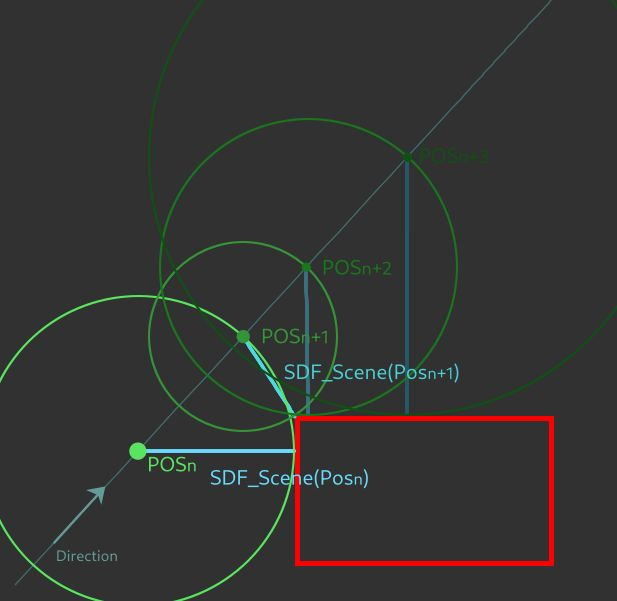
\includegraphics[width=8cm]{images/ProjectionDesRayons.jpg}
    \caption{Illustration 2D de la marche d'un rayon à la position Pos$_n$. Le rectangle rouge est un objet de la scene.}
    \label{fig:projectionrayons}
\end{figure}

\textbf{Remarque} : La suite "avance" dans le sens de \emph{Direction} avec un pas de $SDF\_Scene(Pos_n)$\\
\\
Si la suite \textbf{diverge}, alors le rayon n'a rencontré aucun obstacle. On affichera donc la couleur du ciel.\\
Si la suite \textbf{converge} vers une limite, alors cette limite est le point d'intersection entre la scene 3D et le rayon. On appelera ce point d'intersection le point \textbf{P}.\\
\\
La section suivante explique comment determiner la couleur à afficher dans ce cas là.